\documentclass[twoside]{book}

% Packages required by doxygen
\usepackage{fixltx2e}
\usepackage{calc}
\usepackage{doxygen}
\usepackage[export]{adjustbox} % also loads graphicx
\usepackage{graphicx}
\usepackage[utf8]{inputenc}
\usepackage{makeidx}
\usepackage{multicol}
\usepackage{multirow}
\PassOptionsToPackage{warn}{textcomp}
\usepackage{textcomp}
\usepackage[nointegrals]{wasysym}
\usepackage[table]{xcolor}

% Font selection
\usepackage[T1]{fontenc}
\usepackage[scaled=.90]{helvet}
\usepackage{courier}
\usepackage{amssymb}
\usepackage{sectsty}
\renewcommand{\familydefault}{\sfdefault}
\allsectionsfont{%
  \fontseries{bc}\selectfont%
  \color{darkgray}%
}
\renewcommand{\DoxyLabelFont}{%
  \fontseries{bc}\selectfont%
  \color{darkgray}%
}
\newcommand{\+}{\discretionary{\mbox{\scriptsize$\hookleftarrow$}}{}{}}

% Page & text layout
\usepackage{geometry}
\geometry{%
  a4paper,%
  top=2.5cm,%
  bottom=2.5cm,%
  left=2.5cm,%
  right=2.5cm%
}
\tolerance=750
\hfuzz=15pt
\hbadness=750
\setlength{\emergencystretch}{15pt}
\setlength{\parindent}{0cm}
\setlength{\parskip}{3ex plus 2ex minus 2ex}
\makeatletter
\renewcommand{\paragraph}{%
  \@startsection{paragraph}{4}{0ex}{-1.0ex}{1.0ex}{%
    \normalfont\normalsize\bfseries\SS@parafont%
  }%
}
\renewcommand{\subparagraph}{%
  \@startsection{subparagraph}{5}{0ex}{-1.0ex}{1.0ex}{%
    \normalfont\normalsize\bfseries\SS@subparafont%
  }%
}
\makeatother

% Headers & footers
\usepackage{fancyhdr}
\pagestyle{fancyplain}
\fancyhead[LE]{\fancyplain{}{\bfseries\thepage}}
\fancyhead[CE]{\fancyplain{}{}}
\fancyhead[RE]{\fancyplain{}{\bfseries\leftmark}}
\fancyhead[LO]{\fancyplain{}{\bfseries\rightmark}}
\fancyhead[CO]{\fancyplain{}{}}
\fancyhead[RO]{\fancyplain{}{\bfseries\thepage}}
\fancyfoot[LE]{\fancyplain{}{}}
\fancyfoot[CE]{\fancyplain{}{}}
\fancyfoot[RE]{\fancyplain{}{\bfseries\scriptsize Generated by Doxygen }}
\fancyfoot[LO]{\fancyplain{}{\bfseries\scriptsize Generated by Doxygen }}
\fancyfoot[CO]{\fancyplain{}{}}
\fancyfoot[RO]{\fancyplain{}{}}
\renewcommand{\footrulewidth}{0.4pt}
\renewcommand{\chaptermark}[1]{%
  \markboth{#1}{}%
}
\renewcommand{\sectionmark}[1]{%
  \markright{\thesection\ #1}%
}

% Indices & bibliography
\usepackage{natbib}
\usepackage[titles]{tocloft}
\setcounter{tocdepth}{3}
\setcounter{secnumdepth}{5}
\makeindex

% Hyperlinks (required, but should be loaded last)
\usepackage{ifpdf}
\ifpdf
  \usepackage[pdftex,pagebackref=true]{hyperref}
\else
  \usepackage[ps2pdf,pagebackref=true]{hyperref}
\fi
\hypersetup{%
  colorlinks=true,%
  linkcolor=blue,%
  citecolor=blue,%
  unicode%
}

% Custom commands
\newcommand{\clearemptydoublepage}{%
  \newpage{\pagestyle{empty}\cleardoublepage}%
}

\usepackage{caption}
\captionsetup{labelsep=space,justification=centering,font={bf},singlelinecheck=off,skip=4pt,position=top}

%===== C O N T E N T S =====

\begin{document}

% Titlepage & ToC
\hypersetup{pageanchor=false,
             bookmarksnumbered=true,
             pdfencoding=unicode
            }
\pagenumbering{roman}
\begin{titlepage}
\vspace*{7cm}
\begin{center}%
{\Large Modbus\+\_\+\+L\+P\+C1769 }\\
\vspace*{1cm}
{\large Generated by Doxygen 1.8.11}\\
\end{center}
\end{titlepage}
\clearemptydoublepage
\tableofcontents
\clearemptydoublepage
\pagenumbering{arabic}
\hypersetup{pageanchor=true}

%--- Begin generated contents ---
\chapter{Module Index}
\section{Modules}
Here is a list of all modules\+:\begin{DoxyCompactList}
\item \contentsline{section}{Modbus}{\pageref{group__modbus}}{}
\item \contentsline{section}{Modbus Registers}{\pageref{group__modbus__registers}}{}
\item \contentsline{section}{Modbus Configuration}{\pageref{group__modbus__cfg}}{}
\item \contentsline{section}{Utilities}{\pageref{group__modbus__utils}}{}
\end{DoxyCompactList}

\chapter{Data Structure Index}
\section{Data Structures}
Here are the data structures with brief descriptions\+:\begin{DoxyCompactList}
\item\contentsline{section}{\hyperlink{structx_m_b_function_handler}{x\+M\+B\+Function\+Handler} }{\pageref{structx_m_b_function_handler}}{}
\end{DoxyCompactList}

\chapter{Module Documentation}
\hypertarget{group__modbus}{}\section{Modbus}
\label{group__modbus}\index{Modbus@{Modbus}}
\subsection*{Macros}
\begin{DoxyCompactItemize}
\item 
\#define \hyperlink{group__modbus_ga0e6d79d4ff38dbf7d3fd81a80d655b70}{M\+B\+\_\+\+T\+C\+P\+\_\+\+P\+O\+R\+T\+\_\+\+U\+S\+E\+\_\+\+D\+E\+F\+A\+U\+LT}~0\hypertarget{group__modbus_ga0e6d79d4ff38dbf7d3fd81a80d655b70}{}\label{group__modbus_ga0e6d79d4ff38dbf7d3fd81a80d655b70}

\begin{DoxyCompactList}\small\item\em Use the default Modbus T\+CP port (502) \end{DoxyCompactList}\end{DoxyCompactItemize}
\subsection*{Enumerations}
\begin{DoxyCompactItemize}
\item 
enum \hyperlink{group__modbus_ga462d0d9396f02be6f9fd5b6f19463e61}{e\+M\+B\+Mode} \{ \\*
\hyperlink{group__modbus_gga462d0d9396f02be6f9fd5b6f19463e61a1b807b8cf3d593d8cd8d1a1d21a3da31}{M\+B\+\_\+\+R\+TU}, 
\\*
\hyperlink{group__modbus_gga462d0d9396f02be6f9fd5b6f19463e61afa37751530d5e48cb5a3f8841f9e3143}{M\+B\+\_\+\+A\+S\+C\+II}, 
\\*
\hyperlink{group__modbus_gga462d0d9396f02be6f9fd5b6f19463e61a5786284fe284b4a23889bf5b444d5142}{M\+B\+\_\+\+T\+CP}
 \}\begin{DoxyCompactList}\small\item\em Modbus serial transmission modes (R\+T\+U/\+A\+S\+C\+II). \end{DoxyCompactList}
\item 
enum \hyperlink{group__modbus_gaf1398cbbeb317b1dbd0276b275f5b0f8}{e\+M\+B\+Register\+Mode} \{ \\*
\hyperlink{group__modbus_ggaf1398cbbeb317b1dbd0276b275f5b0f8aa210c1d03e2745efb42486b822740d4b}{M\+B\+\_\+\+R\+E\+G\+\_\+\+R\+E\+AD}, 
\\*
\hyperlink{group__modbus_ggaf1398cbbeb317b1dbd0276b275f5b0f8a3d0a62208562b69c5e7692a5a168c14e}{M\+B\+\_\+\+R\+E\+G\+\_\+\+W\+R\+I\+TE}
 \}\begin{DoxyCompactList}\small\item\em If register should be written or read. \end{DoxyCompactList}
\item 
enum \hyperlink{group__modbus_ga9e7fce8c431cb0e521c67f7f36dd823d}{e\+M\+B\+Error\+Code} \{ \\*
\hyperlink{group__modbus_gga9e7fce8c431cb0e521c67f7f36dd823dabf4c1fb8c72eafc08be972225613fe2b}{M\+B\+\_\+\+E\+N\+O\+E\+RR}, 
\\*
\hyperlink{group__modbus_gga9e7fce8c431cb0e521c67f7f36dd823daf415371aad180c545b726d39adbf9ba7}{M\+B\+\_\+\+E\+N\+O\+R\+EG}, 
\\*
\hyperlink{group__modbus_gga9e7fce8c431cb0e521c67f7f36dd823dafa57cdb3f85e8ab4baf160579104d624}{M\+B\+\_\+\+E\+I\+N\+V\+AL}, 
\\*
\hyperlink{group__modbus_gga9e7fce8c431cb0e521c67f7f36dd823da539fb138411468b12c05556157c6864d}{M\+B\+\_\+\+E\+P\+O\+R\+T\+E\+RR}, 
\\*
\hyperlink{group__modbus_gga9e7fce8c431cb0e521c67f7f36dd823daf0700c1e37bfc75068e6577bc0b04bb8}{M\+B\+\_\+\+E\+N\+O\+R\+ES}, 
\\*
\hyperlink{group__modbus_gga9e7fce8c431cb0e521c67f7f36dd823daf6eed4a1c490af14b7467be1e6e2fe67}{M\+B\+\_\+\+E\+IO}, 
\\*
\hyperlink{group__modbus_gga9e7fce8c431cb0e521c67f7f36dd823daf0e64a209ac1a01935167c6986338a6f}{M\+B\+\_\+\+E\+I\+L\+L\+S\+T\+A\+TE}, 
\\*
\hyperlink{group__modbus_gga9e7fce8c431cb0e521c67f7f36dd823da017c559e956f718cf77aafe269f49bd5}{M\+B\+\_\+\+E\+T\+I\+M\+E\+D\+O\+UT}
 \}\begin{DoxyCompactList}\small\item\em Errorcodes used by all function in the protocol stack. \end{DoxyCompactList}
\item 
enum \hyperlink{group__modbus_ga16ba85fa56bcd52a11a12576af445ccb}{e\+M\+B\+Parity} \{ \\*
\hyperlink{group__modbus_gga16ba85fa56bcd52a11a12576af445ccba36c1b70b68bc05d618632e3f975a557b}{M\+B\+\_\+\+P\+A\+R\+\_\+\+N\+O\+NE}, 
\\*
\hyperlink{group__modbus_gga16ba85fa56bcd52a11a12576af445ccba955fa6c30334314739ddceed6e749316}{M\+B\+\_\+\+P\+A\+R\+\_\+\+O\+DD}, 
\\*
\hyperlink{group__modbus_gga16ba85fa56bcd52a11a12576af445ccba0415f4c7ede57e13a0cca698a8375dbd}{M\+B\+\_\+\+P\+A\+R\+\_\+\+E\+V\+EN}
 \}\begin{DoxyCompactList}\small\item\em Parity used for characters in serial mode. \end{DoxyCompactList}
\end{DoxyCompactItemize}
\subsection*{Functions}
\begin{DoxyCompactItemize}
\item 
\hyperlink{group__modbus_ga9e7fce8c431cb0e521c67f7f36dd823d}{e\+M\+B\+Error\+Code} \hyperlink{group__modbus_ga622dbe6b38ff1d255523d4736fa3da26}{e\+M\+B\+Init} (\hyperlink{group__modbus_ga462d0d9396f02be6f9fd5b6f19463e61}{e\+M\+B\+Mode} e\+Mode, U\+C\+H\+AR uc\+Slave\+Address, U\+C\+H\+AR uc\+Port, U\+L\+O\+NG ul\+Baud\+Rate, \hyperlink{group__modbus_ga16ba85fa56bcd52a11a12576af445ccb}{e\+M\+B\+Parity} e\+Parity)
\begin{DoxyCompactList}\small\item\em Initialize the Modbus protocol stack. \end{DoxyCompactList}\item 
\hyperlink{group__modbus_ga9e7fce8c431cb0e521c67f7f36dd823d}{e\+M\+B\+Error\+Code} \hyperlink{group__modbus_gab06a2d0ef8bdfd866cd934f0ec7e7a6e}{e\+M\+B\+T\+C\+P\+Init} (U\+S\+H\+O\+RT us\+T\+C\+P\+Port)
\begin{DoxyCompactList}\small\item\em Initialize the Modbus protocol stack for Modbus T\+CP. \end{DoxyCompactList}\item 
\hyperlink{group__modbus_ga9e7fce8c431cb0e521c67f7f36dd823d}{e\+M\+B\+Error\+Code} \hyperlink{group__modbus_gac20080d92be2934456e2a5d27cd36310}{e\+M\+B\+Close} (void)
\begin{DoxyCompactList}\small\item\em Release resources used by the protocol stack. \end{DoxyCompactList}\item 
\hyperlink{group__modbus_ga9e7fce8c431cb0e521c67f7f36dd823d}{e\+M\+B\+Error\+Code} \hyperlink{group__modbus_gab697be370833d562e6b016626d996132}{e\+M\+B\+Enable} (void)
\begin{DoxyCompactList}\small\item\em Enable the Modbus protocol stack. \end{DoxyCompactList}\item 
\hyperlink{group__modbus_ga9e7fce8c431cb0e521c67f7f36dd823d}{e\+M\+B\+Error\+Code} \hyperlink{group__modbus_gabcc2a31ec41fc276ab3c3ac705defdf3}{e\+M\+B\+Disable} (void)
\begin{DoxyCompactList}\small\item\em Disable the Modbus protocol stack. \end{DoxyCompactList}\item 
\hyperlink{group__modbus_ga9e7fce8c431cb0e521c67f7f36dd823d}{e\+M\+B\+Error\+Code} \hyperlink{group__modbus_ga12648c98d45f768ba878fbcee46caca5}{e\+M\+B\+Poll} (void)
\begin{DoxyCompactList}\small\item\em The main pooling loop of the Modbus protocol stack. \end{DoxyCompactList}\item 
\hyperlink{group__modbus_ga9e7fce8c431cb0e521c67f7f36dd823d}{e\+M\+B\+Error\+Code} \hyperlink{group__modbus_gabe2b0e2dccf23d506666aa3cfdf6a8a3}{e\+M\+B\+Set\+Slave\+ID} (U\+C\+H\+AR uc\+Slave\+ID, B\+O\+OL x\+Is\+Running, U\+C\+H\+AR const $\ast$puc\+Additional, U\+S\+H\+O\+RT us\+Additional\+Len)
\begin{DoxyCompactList}\small\item\em Configure the slave id of the device. \end{DoxyCompactList}\item 
\hyperlink{group__modbus_ga9e7fce8c431cb0e521c67f7f36dd823d}{e\+M\+B\+Error\+Code} \hyperlink{group__modbus_ga5f6e66893b2388a602ac453253a00784}{e\+M\+B\+Register\+CB} (U\+C\+H\+AR uc\+Function\+Code, px\+M\+B\+Function\+Handler px\+Handler)
\begin{DoxyCompactList}\small\item\em Registers a callback handler for a given function code. \end{DoxyCompactList}\end{DoxyCompactItemize}


\subsection{Detailed Description}

\begin{DoxyCode}
\textcolor{preprocessor}{#include "mb.h"} 
\end{DoxyCode}


This module defines the interface for the application. It contains the basic functions and types required to use the Modbus protocol stack. A typical application will want to call \hyperlink{group__modbus_ga622dbe6b38ff1d255523d4736fa3da26}{e\+M\+B\+Init()} first. If the device is ready to answer network requests it must then call \hyperlink{group__modbus_gab697be370833d562e6b016626d996132}{e\+M\+B\+Enable()} to activate the protocol stack. In the main loop the function \hyperlink{group__modbus_ga12648c98d45f768ba878fbcee46caca5}{e\+M\+B\+Poll()} must be called periodically. The time interval between pooling depends on the configured Modbus timeout. If an R\+T\+OS is available a separate task should be created and the task should always call the function \hyperlink{group__modbus_ga12648c98d45f768ba878fbcee46caca5}{e\+M\+B\+Poll()}.


\begin{DoxyCode}
\textcolor{comment}{// Initialize protocol stack in RTU mode for a slave with address 10 = 0x0A}
\hyperlink{group__modbus_ga622dbe6b38ff1d255523d4736fa3da26}{eMBInit}( \hyperlink{group__modbus_gga462d0d9396f02be6f9fd5b6f19463e61a1b807b8cf3d593d8cd8d1a1d21a3da31}{MB\_RTU}, 0x0A, 38400, \hyperlink{group__modbus_gga16ba85fa56bcd52a11a12576af445ccba0415f4c7ede57e13a0cca698a8375dbd}{MB\_PAR\_EVEN} );
\textcolor{comment}{// Enable the Modbus Protocol Stack.}
\hyperlink{group__modbus_gab697be370833d562e6b016626d996132}{eMBEnable}(  );
\textcolor{keywordflow}{for}( ;; )
\{
    \textcolor{comment}{// Call the main polling loop of the Modbus protocol stack.}
    \hyperlink{group__modbus_ga12648c98d45f768ba878fbcee46caca5}{eMBPoll}(  );
    ...
\}
\end{DoxyCode}
 

\subsection{Enumeration Type Documentation}
\index{Modbus@{Modbus}!e\+M\+B\+Mode@{e\+M\+B\+Mode}}
\index{e\+M\+B\+Mode@{e\+M\+B\+Mode}!Modbus@{Modbus}}
\subsubsection[{\texorpdfstring{e\+M\+B\+Mode}{eMBMode}}]{\setlength{\rightskip}{0pt plus 5cm}enum {\bf e\+M\+B\+Mode}}\hypertarget{group__modbus_ga462d0d9396f02be6f9fd5b6f19463e61}{}\label{group__modbus_ga462d0d9396f02be6f9fd5b6f19463e61}


Modbus serial transmission modes (R\+T\+U/\+A\+S\+C\+II). 

Modbus serial supports two transmission modes. Either A\+S\+C\+II or R\+TU. R\+TU is faster but has more hardware requirements and requires a network with a low jitter. A\+S\+C\+II is slower and more reliable on slower links (E.\+g. modems) \begin{Desc}
\item[Enumerator]\par
\begin{description}
\index{M\+B\+\_\+\+R\+TU@{M\+B\+\_\+\+R\+TU}!Modbus@{Modbus}}\index{Modbus@{Modbus}!M\+B\+\_\+\+R\+TU@{M\+B\+\_\+\+R\+TU}}\item[{\em 
M\+B\+\_\+\+R\+TU\hypertarget{group__modbus_gga462d0d9396f02be6f9fd5b6f19463e61a1b807b8cf3d593d8cd8d1a1d21a3da31}{}\label{group__modbus_gga462d0d9396f02be6f9fd5b6f19463e61a1b807b8cf3d593d8cd8d1a1d21a3da31}
}]R\+TU transmission mode. \index{M\+B\+\_\+\+A\+S\+C\+II@{M\+B\+\_\+\+A\+S\+C\+II}!Modbus@{Modbus}}\index{Modbus@{Modbus}!M\+B\+\_\+\+A\+S\+C\+II@{M\+B\+\_\+\+A\+S\+C\+II}}\item[{\em 
M\+B\+\_\+\+A\+S\+C\+II\hypertarget{group__modbus_gga462d0d9396f02be6f9fd5b6f19463e61afa37751530d5e48cb5a3f8841f9e3143}{}\label{group__modbus_gga462d0d9396f02be6f9fd5b6f19463e61afa37751530d5e48cb5a3f8841f9e3143}
}]A\+S\+C\+II transmission mode. \index{M\+B\+\_\+\+T\+CP@{M\+B\+\_\+\+T\+CP}!Modbus@{Modbus}}\index{Modbus@{Modbus}!M\+B\+\_\+\+T\+CP@{M\+B\+\_\+\+T\+CP}}\item[{\em 
M\+B\+\_\+\+T\+CP\hypertarget{group__modbus_gga462d0d9396f02be6f9fd5b6f19463e61a5786284fe284b4a23889bf5b444d5142}{}\label{group__modbus_gga462d0d9396f02be6f9fd5b6f19463e61a5786284fe284b4a23889bf5b444d5142}
}]T\+CP mode. \end{description}
\end{Desc}


Definition at line 85 of file mb.\+h.

\index{Modbus@{Modbus}!e\+M\+B\+Register\+Mode@{e\+M\+B\+Register\+Mode}}
\index{e\+M\+B\+Register\+Mode@{e\+M\+B\+Register\+Mode}!Modbus@{Modbus}}
\subsubsection[{\texorpdfstring{e\+M\+B\+Register\+Mode}{eMBRegisterMode}}]{\setlength{\rightskip}{0pt plus 5cm}enum {\bf e\+M\+B\+Register\+Mode}}\hypertarget{group__modbus_gaf1398cbbeb317b1dbd0276b275f5b0f8}{}\label{group__modbus_gaf1398cbbeb317b1dbd0276b275f5b0f8}


If register should be written or read. 

This value is passed to the callback functions which support either reading or writing register values. Writing means that the application registers should be updated and reading means that the modbus protocol stack needs to know the current register values.

\begin{DoxySeeAlso}{See also}
\hyperlink{group__modbus__registers_ga10d37e1d80224bf3b1eeb9e246d7582e}{e\+M\+B\+Reg\+Holding\+C\+B( )}, \hyperlink{group__modbus__registers_ga88d9b719291515c60eee1bf9ffa1dd02}{e\+M\+B\+Reg\+Coils\+C\+B( )}, \hyperlink{group__modbus__registers_ga38101f5da54af137e210a3b8b9fa3887}{e\+M\+B\+Reg\+Discrete\+C\+B( )} and \hyperlink{group__modbus__registers_ga7816677520b1eb2ebecf15060a41bc81}{e\+M\+B\+Reg\+Input\+C\+B( )}. 
\end{DoxySeeAlso}
\begin{Desc}
\item[Enumerator]\par
\begin{description}
\index{M\+B\+\_\+\+R\+E\+G\+\_\+\+R\+E\+AD@{M\+B\+\_\+\+R\+E\+G\+\_\+\+R\+E\+AD}!Modbus@{Modbus}}\index{Modbus@{Modbus}!M\+B\+\_\+\+R\+E\+G\+\_\+\+R\+E\+AD@{M\+B\+\_\+\+R\+E\+G\+\_\+\+R\+E\+AD}}\item[{\em 
M\+B\+\_\+\+R\+E\+G\+\_\+\+R\+E\+AD\hypertarget{group__modbus_ggaf1398cbbeb317b1dbd0276b275f5b0f8aa210c1d03e2745efb42486b822740d4b}{}\label{group__modbus_ggaf1398cbbeb317b1dbd0276b275f5b0f8aa210c1d03e2745efb42486b822740d4b}
}]Read register values and pass to protocol stack. \index{M\+B\+\_\+\+R\+E\+G\+\_\+\+W\+R\+I\+TE@{M\+B\+\_\+\+R\+E\+G\+\_\+\+W\+R\+I\+TE}!Modbus@{Modbus}}\index{Modbus@{Modbus}!M\+B\+\_\+\+R\+E\+G\+\_\+\+W\+R\+I\+TE@{M\+B\+\_\+\+R\+E\+G\+\_\+\+W\+R\+I\+TE}}\item[{\em 
M\+B\+\_\+\+R\+E\+G\+\_\+\+W\+R\+I\+TE\hypertarget{group__modbus_ggaf1398cbbeb317b1dbd0276b275f5b0f8a3d0a62208562b69c5e7692a5a168c14e}{}\label{group__modbus_ggaf1398cbbeb317b1dbd0276b275f5b0f8a3d0a62208562b69c5e7692a5a168c14e}
}]Update register values. \end{description}
\end{Desc}


Definition at line 103 of file mb.\+h.

\index{Modbus@{Modbus}!e\+M\+B\+Error\+Code@{e\+M\+B\+Error\+Code}}
\index{e\+M\+B\+Error\+Code@{e\+M\+B\+Error\+Code}!Modbus@{Modbus}}
\subsubsection[{\texorpdfstring{e\+M\+B\+Error\+Code}{eMBErrorCode}}]{\setlength{\rightskip}{0pt plus 5cm}enum {\bf e\+M\+B\+Error\+Code}}\hypertarget{group__modbus_ga9e7fce8c431cb0e521c67f7f36dd823d}{}\label{group__modbus_ga9e7fce8c431cb0e521c67f7f36dd823d}


Errorcodes used by all function in the protocol stack. 

\begin{Desc}
\item[Enumerator]\par
\begin{description}
\index{M\+B\+\_\+\+E\+N\+O\+E\+RR@{M\+B\+\_\+\+E\+N\+O\+E\+RR}!Modbus@{Modbus}}\index{Modbus@{Modbus}!M\+B\+\_\+\+E\+N\+O\+E\+RR@{M\+B\+\_\+\+E\+N\+O\+E\+RR}}\item[{\em 
M\+B\+\_\+\+E\+N\+O\+E\+RR\hypertarget{group__modbus_gga9e7fce8c431cb0e521c67f7f36dd823dabf4c1fb8c72eafc08be972225613fe2b}{}\label{group__modbus_gga9e7fce8c431cb0e521c67f7f36dd823dabf4c1fb8c72eafc08be972225613fe2b}
}]no error. \index{M\+B\+\_\+\+E\+N\+O\+R\+EG@{M\+B\+\_\+\+E\+N\+O\+R\+EG}!Modbus@{Modbus}}\index{Modbus@{Modbus}!M\+B\+\_\+\+E\+N\+O\+R\+EG@{M\+B\+\_\+\+E\+N\+O\+R\+EG}}\item[{\em 
M\+B\+\_\+\+E\+N\+O\+R\+EG\hypertarget{group__modbus_gga9e7fce8c431cb0e521c67f7f36dd823daf415371aad180c545b726d39adbf9ba7}{}\label{group__modbus_gga9e7fce8c431cb0e521c67f7f36dd823daf415371aad180c545b726d39adbf9ba7}
}]illegal register address. \index{M\+B\+\_\+\+E\+I\+N\+V\+AL@{M\+B\+\_\+\+E\+I\+N\+V\+AL}!Modbus@{Modbus}}\index{Modbus@{Modbus}!M\+B\+\_\+\+E\+I\+N\+V\+AL@{M\+B\+\_\+\+E\+I\+N\+V\+AL}}\item[{\em 
M\+B\+\_\+\+E\+I\+N\+V\+AL\hypertarget{group__modbus_gga9e7fce8c431cb0e521c67f7f36dd823dafa57cdb3f85e8ab4baf160579104d624}{}\label{group__modbus_gga9e7fce8c431cb0e521c67f7f36dd823dafa57cdb3f85e8ab4baf160579104d624}
}]illegal argument. \index{M\+B\+\_\+\+E\+P\+O\+R\+T\+E\+RR@{M\+B\+\_\+\+E\+P\+O\+R\+T\+E\+RR}!Modbus@{Modbus}}\index{Modbus@{Modbus}!M\+B\+\_\+\+E\+P\+O\+R\+T\+E\+RR@{M\+B\+\_\+\+E\+P\+O\+R\+T\+E\+RR}}\item[{\em 
M\+B\+\_\+\+E\+P\+O\+R\+T\+E\+RR\hypertarget{group__modbus_gga9e7fce8c431cb0e521c67f7f36dd823da539fb138411468b12c05556157c6864d}{}\label{group__modbus_gga9e7fce8c431cb0e521c67f7f36dd823da539fb138411468b12c05556157c6864d}
}]porting layer error. \index{M\+B\+\_\+\+E\+N\+O\+R\+ES@{M\+B\+\_\+\+E\+N\+O\+R\+ES}!Modbus@{Modbus}}\index{Modbus@{Modbus}!M\+B\+\_\+\+E\+N\+O\+R\+ES@{M\+B\+\_\+\+E\+N\+O\+R\+ES}}\item[{\em 
M\+B\+\_\+\+E\+N\+O\+R\+ES\hypertarget{group__modbus_gga9e7fce8c431cb0e521c67f7f36dd823daf0700c1e37bfc75068e6577bc0b04bb8}{}\label{group__modbus_gga9e7fce8c431cb0e521c67f7f36dd823daf0700c1e37bfc75068e6577bc0b04bb8}
}]insufficient resources. \index{M\+B\+\_\+\+E\+IO@{M\+B\+\_\+\+E\+IO}!Modbus@{Modbus}}\index{Modbus@{Modbus}!M\+B\+\_\+\+E\+IO@{M\+B\+\_\+\+E\+IO}}\item[{\em 
M\+B\+\_\+\+E\+IO\hypertarget{group__modbus_gga9e7fce8c431cb0e521c67f7f36dd823daf6eed4a1c490af14b7467be1e6e2fe67}{}\label{group__modbus_gga9e7fce8c431cb0e521c67f7f36dd823daf6eed4a1c490af14b7467be1e6e2fe67}
}]I/O error. \index{M\+B\+\_\+\+E\+I\+L\+L\+S\+T\+A\+TE@{M\+B\+\_\+\+E\+I\+L\+L\+S\+T\+A\+TE}!Modbus@{Modbus}}\index{Modbus@{Modbus}!M\+B\+\_\+\+E\+I\+L\+L\+S\+T\+A\+TE@{M\+B\+\_\+\+E\+I\+L\+L\+S\+T\+A\+TE}}\item[{\em 
M\+B\+\_\+\+E\+I\+L\+L\+S\+T\+A\+TE\hypertarget{group__modbus_gga9e7fce8c431cb0e521c67f7f36dd823daf0e64a209ac1a01935167c6986338a6f}{}\label{group__modbus_gga9e7fce8c431cb0e521c67f7f36dd823daf0e64a209ac1a01935167c6986338a6f}
}]protocol stack in illegal state. \index{M\+B\+\_\+\+E\+T\+I\+M\+E\+D\+O\+UT@{M\+B\+\_\+\+E\+T\+I\+M\+E\+D\+O\+UT}!Modbus@{Modbus}}\index{Modbus@{Modbus}!M\+B\+\_\+\+E\+T\+I\+M\+E\+D\+O\+UT@{M\+B\+\_\+\+E\+T\+I\+M\+E\+D\+O\+UT}}\item[{\em 
M\+B\+\_\+\+E\+T\+I\+M\+E\+D\+O\+UT\hypertarget{group__modbus_gga9e7fce8c431cb0e521c67f7f36dd823da017c559e956f718cf77aafe269f49bd5}{}\label{group__modbus_gga9e7fce8c431cb0e521c67f7f36dd823da017c559e956f718cf77aafe269f49bd5}
}]timeout error occurred. \end{description}
\end{Desc}


Definition at line 112 of file mb.\+h.

\index{Modbus@{Modbus}!e\+M\+B\+Parity@{e\+M\+B\+Parity}}
\index{e\+M\+B\+Parity@{e\+M\+B\+Parity}!Modbus@{Modbus}}
\subsubsection[{\texorpdfstring{e\+M\+B\+Parity}{eMBParity}}]{\setlength{\rightskip}{0pt plus 5cm}enum {\bf e\+M\+B\+Parity}}\hypertarget{group__modbus_ga16ba85fa56bcd52a11a12576af445ccb}{}\label{group__modbus_ga16ba85fa56bcd52a11a12576af445ccb}


Parity used for characters in serial mode. 

The parity which should be applied to the characters sent over the serial link. Please note that this values are actually passed to the porting layer and therefore not all parity modes might be available. \begin{Desc}
\item[Enumerator]\par
\begin{description}
\index{M\+B\+\_\+\+P\+A\+R\+\_\+\+N\+O\+NE@{M\+B\+\_\+\+P\+A\+R\+\_\+\+N\+O\+NE}!Modbus@{Modbus}}\index{Modbus@{Modbus}!M\+B\+\_\+\+P\+A\+R\+\_\+\+N\+O\+NE@{M\+B\+\_\+\+P\+A\+R\+\_\+\+N\+O\+NE}}\item[{\em 
M\+B\+\_\+\+P\+A\+R\+\_\+\+N\+O\+NE\hypertarget{group__modbus_gga16ba85fa56bcd52a11a12576af445ccba36c1b70b68bc05d618632e3f975a557b}{}\label{group__modbus_gga16ba85fa56bcd52a11a12576af445ccba36c1b70b68bc05d618632e3f975a557b}
}]No parity. \index{M\+B\+\_\+\+P\+A\+R\+\_\+\+O\+DD@{M\+B\+\_\+\+P\+A\+R\+\_\+\+O\+DD}!Modbus@{Modbus}}\index{Modbus@{Modbus}!M\+B\+\_\+\+P\+A\+R\+\_\+\+O\+DD@{M\+B\+\_\+\+P\+A\+R\+\_\+\+O\+DD}}\item[{\em 
M\+B\+\_\+\+P\+A\+R\+\_\+\+O\+DD\hypertarget{group__modbus_gga16ba85fa56bcd52a11a12576af445ccba955fa6c30334314739ddceed6e749316}{}\label{group__modbus_gga16ba85fa56bcd52a11a12576af445ccba955fa6c30334314739ddceed6e749316}
}]Odd parity. \index{M\+B\+\_\+\+P\+A\+R\+\_\+\+E\+V\+EN@{M\+B\+\_\+\+P\+A\+R\+\_\+\+E\+V\+EN}!Modbus@{Modbus}}\index{Modbus@{Modbus}!M\+B\+\_\+\+P\+A\+R\+\_\+\+E\+V\+EN@{M\+B\+\_\+\+P\+A\+R\+\_\+\+E\+V\+EN}}\item[{\em 
M\+B\+\_\+\+P\+A\+R\+\_\+\+E\+V\+EN\hypertarget{group__modbus_gga16ba85fa56bcd52a11a12576af445ccba0415f4c7ede57e13a0cca698a8375dbd}{}\label{group__modbus_gga16ba85fa56bcd52a11a12576af445ccba0415f4c7ede57e13a0cca698a8375dbd}
}]Even parity. \end{description}
\end{Desc}


Definition at line 55 of file mbport.\+h.



\subsection{Function Documentation}
\index{Modbus@{Modbus}!e\+M\+B\+Init@{e\+M\+B\+Init}}
\index{e\+M\+B\+Init@{e\+M\+B\+Init}!Modbus@{Modbus}}
\subsubsection[{\texorpdfstring{e\+M\+B\+Init(e\+M\+B\+Mode e\+Mode, U\+C\+H\+A\+R uc\+Slave\+Address, U\+C\+H\+A\+R uc\+Port, U\+L\+O\+N\+G ul\+Baud\+Rate, e\+M\+B\+Parity e\+Parity)}{eMBInit(eMBMode eMode, UCHAR ucSlaveAddress, UCHAR ucPort, ULONG ulBaudRate, eMBParity eParity)}}]{\setlength{\rightskip}{0pt plus 5cm}{\bf e\+M\+B\+Error\+Code} e\+M\+B\+Init (
\begin{DoxyParamCaption}
\item[{{\bf e\+M\+B\+Mode}}]{e\+Mode, }
\item[{U\+C\+H\+AR}]{uc\+Slave\+Address, }
\item[{U\+C\+H\+AR}]{uc\+Port, }
\item[{U\+L\+O\+NG}]{ul\+Baud\+Rate, }
\item[{{\bf e\+M\+B\+Parity}}]{e\+Parity}
\end{DoxyParamCaption}
)}\hypertarget{group__modbus_ga622dbe6b38ff1d255523d4736fa3da26}{}\label{group__modbus_ga622dbe6b38ff1d255523d4736fa3da26}


Initialize the Modbus protocol stack. 

This functions initializes the A\+S\+C\+II or R\+TU module and calls the init functions of the porting layer to prepare the hardware. Please note that the receiver is still disabled and no Modbus frames are processed until \hyperlink{group__modbus_gab697be370833d562e6b016626d996132}{e\+M\+B\+Enable( )} has been called.


\begin{DoxyParams}{Parameters}
{\em e\+Mode} & If A\+S\+C\+II or R\+TU mode should be used. \\
\hline
{\em uc\+Slave\+Address} & The slave address. Only frames sent to this address or to the broadcast address are processed. \\
\hline
{\em uc\+Port} & The port to use. E.\+g. 1 for C\+O\+M1 on windows. This value is platform dependent and some ports simply choose to ignore it. \\
\hline
{\em ul\+Baud\+Rate} & The baudrate. E.\+g. 19200. Supported baudrates depend on the porting layer. \\
\hline
{\em e\+Parity} & Parity used for serial transmission.\\
\hline
\end{DoxyParams}
\begin{DoxyReturn}{Returns}
If no error occurs the function returns e\+M\+B\+Error\+Code\+::\+M\+B\+\_\+\+E\+N\+O\+E\+RR. The protocol is then in the disabled state and ready for activation by calling \hyperlink{group__modbus_gab697be370833d562e6b016626d996132}{e\+M\+B\+Enable( )}. Otherwise one of the following error codes is returned\+:
\begin{DoxyItemize}
\item e\+M\+B\+Error\+Code\+::\+M\+B\+\_\+\+E\+I\+N\+V\+AL If the slave address was not valid. Valid slave addresses are in the range 1 -\/ 247.
\item e\+M\+B\+Error\+Code\+::\+M\+B\+\_\+\+E\+P\+O\+R\+T\+E\+RR IF the porting layer returned an error. 
\end{DoxyItemize}
\end{DoxyReturn}


Definition at line 128 of file mb.\+c.



Here is the call graph for this function\+:\nopagebreak
\begin{figure}[H]
\begin{center}
\leavevmode
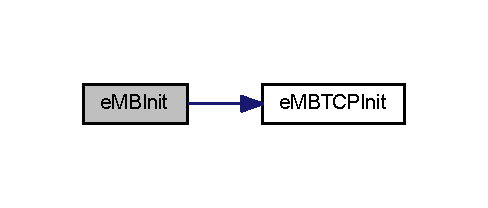
\includegraphics[width=234pt]{group__modbus_ga622dbe6b38ff1d255523d4736fa3da26_cgraph}
\end{center}
\end{figure}


\index{Modbus@{Modbus}!e\+M\+B\+T\+C\+P\+Init@{e\+M\+B\+T\+C\+P\+Init}}
\index{e\+M\+B\+T\+C\+P\+Init@{e\+M\+B\+T\+C\+P\+Init}!Modbus@{Modbus}}
\subsubsection[{\texorpdfstring{e\+M\+B\+T\+C\+P\+Init(\+U\+S\+H\+O\+R\+T us\+T\+C\+P\+Port)}{eMBTCPInit(USHORT usTCPPort)}}]{\setlength{\rightskip}{0pt plus 5cm}{\bf e\+M\+B\+Error\+Code} e\+M\+B\+T\+C\+P\+Init (
\begin{DoxyParamCaption}
\item[{U\+S\+H\+O\+RT}]{us\+T\+C\+P\+Port}
\end{DoxyParamCaption}
)}\hypertarget{group__modbus_gab06a2d0ef8bdfd866cd934f0ec7e7a6e}{}\label{group__modbus_gab06a2d0ef8bdfd866cd934f0ec7e7a6e}


Initialize the Modbus protocol stack for Modbus T\+CP. 

This function initializes the Modbus T\+CP Module. Please note that frame processing is still disabled until \hyperlink{group__modbus_gab697be370833d562e6b016626d996132}{e\+M\+B\+Enable( )} is called.


\begin{DoxyParams}{Parameters}
{\em us\+T\+C\+P\+Port} & The T\+CP port to listen on. \\
\hline
\end{DoxyParams}
\begin{DoxyReturn}{Returns}
If the protocol stack has been initialized correctly the function returns e\+M\+B\+Error\+Code\+::\+M\+B\+\_\+\+E\+N\+O\+E\+RR. Otherwise one of the following error codes is returned\+:
\begin{DoxyItemize}
\item e\+M\+B\+Error\+Code\+::\+M\+B\+\_\+\+E\+I\+N\+V\+AL If the slave address was not valid. Valid slave addresses are in the range 1 -\/ 247.
\item e\+M\+B\+Error\+Code\+::\+M\+B\+\_\+\+E\+P\+O\+R\+T\+E\+RR IF the porting layer returned an error. 
\end{DoxyItemize}
\end{DoxyReturn}


Here is the caller graph for this function\+:\nopagebreak
\begin{figure}[H]
\begin{center}
\leavevmode
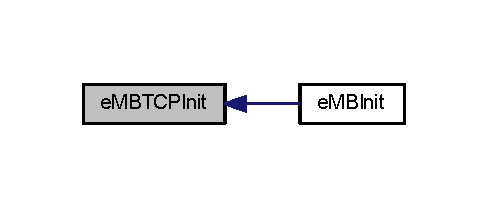
\includegraphics[width=234pt]{group__modbus_gab06a2d0ef8bdfd866cd934f0ec7e7a6e_icgraph}
\end{center}
\end{figure}


\index{Modbus@{Modbus}!e\+M\+B\+Close@{e\+M\+B\+Close}}
\index{e\+M\+B\+Close@{e\+M\+B\+Close}!Modbus@{Modbus}}
\subsubsection[{\texorpdfstring{e\+M\+B\+Close(void)}{eMBClose(void)}}]{\setlength{\rightskip}{0pt plus 5cm}{\bf e\+M\+B\+Error\+Code} e\+M\+B\+Close (
\begin{DoxyParamCaption}
\item[{void}]{}
\end{DoxyParamCaption}
)}\hypertarget{group__modbus_gac20080d92be2934456e2a5d27cd36310}{}\label{group__modbus_gac20080d92be2934456e2a5d27cd36310}


Release resources used by the protocol stack. 

This function disables the Modbus protocol stack and release all hardware resources. It must only be called when the protocol stack is disabled.

\begin{DoxyNote}{Note}
Note all ports implement this function. A port which wants to get an callback must define the macro M\+B\+\_\+\+P\+O\+R\+T\+\_\+\+H\+A\+S\+\_\+\+C\+L\+O\+SE to 1.
\end{DoxyNote}
\begin{DoxyReturn}{Returns}
If the resources where released it return e\+M\+B\+Error\+Code\+::\+M\+B\+\_\+\+E\+N\+O\+E\+RR. If the protocol stack is not in the disabled state it returns e\+M\+B\+Error\+Code\+::\+M\+B\+\_\+\+E\+I\+L\+L\+S\+T\+A\+TE. 
\end{DoxyReturn}


Definition at line 265 of file mb.\+c.

\index{Modbus@{Modbus}!e\+M\+B\+Enable@{e\+M\+B\+Enable}}
\index{e\+M\+B\+Enable@{e\+M\+B\+Enable}!Modbus@{Modbus}}
\subsubsection[{\texorpdfstring{e\+M\+B\+Enable(void)}{eMBEnable(void)}}]{\setlength{\rightskip}{0pt plus 5cm}{\bf e\+M\+B\+Error\+Code} e\+M\+B\+Enable (
\begin{DoxyParamCaption}
\item[{void}]{}
\end{DoxyParamCaption}
)}\hypertarget{group__modbus_gab697be370833d562e6b016626d996132}{}\label{group__modbus_gab697be370833d562e6b016626d996132}


Enable the Modbus protocol stack. 

This function enables processing of Modbus frames. Enabling the protocol stack is only possible if it is in the disabled state.

\begin{DoxyReturn}{Returns}
If the protocol stack is now in the state enabled it returns e\+M\+B\+Error\+Code\+::\+M\+B\+\_\+\+E\+N\+O\+E\+RR. If it was not in the disabled state it return e\+M\+B\+Error\+Code\+::\+M\+B\+\_\+\+E\+I\+L\+L\+S\+T\+A\+TE. 
\end{DoxyReturn}


Definition at line 284 of file mb.\+c.

\index{Modbus@{Modbus}!e\+M\+B\+Disable@{e\+M\+B\+Disable}}
\index{e\+M\+B\+Disable@{e\+M\+B\+Disable}!Modbus@{Modbus}}
\subsubsection[{\texorpdfstring{e\+M\+B\+Disable(void)}{eMBDisable(void)}}]{\setlength{\rightskip}{0pt plus 5cm}{\bf e\+M\+B\+Error\+Code} e\+M\+B\+Disable (
\begin{DoxyParamCaption}
\item[{void}]{}
\end{DoxyParamCaption}
)}\hypertarget{group__modbus_gabcc2a31ec41fc276ab3c3ac705defdf3}{}\label{group__modbus_gabcc2a31ec41fc276ab3c3ac705defdf3}


Disable the Modbus protocol stack. 

This function disables processing of Modbus frames.

\begin{DoxyReturn}{Returns}
If the protocol stack has been disabled it returns e\+M\+B\+Error\+Code\+::\+M\+B\+\_\+\+E\+N\+O\+E\+RR. If it was not in the enabled state it returns e\+M\+B\+Error\+Code\+::\+M\+B\+\_\+\+E\+I\+L\+L\+S\+T\+A\+TE. 
\end{DoxyReturn}


Definition at line 302 of file mb.\+c.

\index{Modbus@{Modbus}!e\+M\+B\+Poll@{e\+M\+B\+Poll}}
\index{e\+M\+B\+Poll@{e\+M\+B\+Poll}!Modbus@{Modbus}}
\subsubsection[{\texorpdfstring{e\+M\+B\+Poll(void)}{eMBPoll(void)}}]{\setlength{\rightskip}{0pt plus 5cm}{\bf e\+M\+B\+Error\+Code} e\+M\+B\+Poll (
\begin{DoxyParamCaption}
\item[{void}]{}
\end{DoxyParamCaption}
)}\hypertarget{group__modbus_ga12648c98d45f768ba878fbcee46caca5}{}\label{group__modbus_ga12648c98d45f768ba878fbcee46caca5}


The main pooling loop of the Modbus protocol stack. 

This function must be called periodically. The timer interval required is given by the application dependent Modbus slave timeout. Internally the function calls x\+M\+B\+Port\+Event\+Get() and waits for an event from the receiver or transmitter state machines.

\begin{DoxyReturn}{Returns}
If the protocol stack is not in the enabled state the function returns e\+M\+B\+Error\+Code\+::\+M\+B\+\_\+\+E\+I\+L\+L\+S\+T\+A\+TE. Otherwise it returns e\+M\+B\+Error\+Code\+::\+M\+B\+\_\+\+E\+N\+O\+E\+RR. 
\end{DoxyReturn}


Definition at line 324 of file mb.\+c.

\index{Modbus@{Modbus}!e\+M\+B\+Set\+Slave\+ID@{e\+M\+B\+Set\+Slave\+ID}}
\index{e\+M\+B\+Set\+Slave\+ID@{e\+M\+B\+Set\+Slave\+ID}!Modbus@{Modbus}}
\subsubsection[{\texorpdfstring{e\+M\+B\+Set\+Slave\+I\+D(\+U\+C\+H\+A\+R uc\+Slave\+I\+D, B\+O\+O\+L x\+Is\+Running, U\+C\+H\+A\+R const $\ast$puc\+Additional, U\+S\+H\+O\+R\+T us\+Additional\+Len)}{eMBSetSlaveID(UCHAR ucSlaveID, BOOL xIsRunning, UCHAR const *pucAdditional, USHORT usAdditionalLen)}}]{\setlength{\rightskip}{0pt plus 5cm}{\bf e\+M\+B\+Error\+Code} e\+M\+B\+Set\+Slave\+ID (
\begin{DoxyParamCaption}
\item[{U\+C\+H\+AR}]{uc\+Slave\+ID, }
\item[{B\+O\+OL}]{x\+Is\+Running, }
\item[{U\+C\+H\+AR const $\ast$}]{puc\+Additional, }
\item[{U\+S\+H\+O\+RT}]{us\+Additional\+Len}
\end{DoxyParamCaption}
)}\hypertarget{group__modbus_gabe2b0e2dccf23d506666aa3cfdf6a8a3}{}\label{group__modbus_gabe2b0e2dccf23d506666aa3cfdf6a8a3}


Configure the slave id of the device. 

This function should be called when the Modbus function {\itshape Report Slave ID} is enabled ( By defining M\+B\+\_\+\+F\+U\+N\+C\+\_\+\+O\+T\+H\+E\+R\+\_\+\+R\+E\+P\+\_\+\+S\+L\+A\+V\+E\+I\+D\+\_\+\+E\+N\+A\+B\+L\+ED in \hyperlink{mbconfig_8h_source}{mbconfig.\+h} ).


\begin{DoxyParams}{Parameters}
{\em uc\+Slave\+ID} & Values is returned in the {\itshape Slave ID} byte of the {\itshape Report Slave ID} response. \\
\hline
{\em x\+Is\+Running} & If T\+R\+UE the {\itshape Run Indicator Status} byte is set to 0x\+FF. otherwise the {\itshape Run Indicator Status} is 0x00. \\
\hline
{\em puc\+Additional} & Values which should be returned in the {\itshape Additional} bytes of the {\itshape  Report Slave ID} response. \\
\hline
{\em us\+Additional\+Len} & Length of the buffer {\ttfamily puc\+Additonal}.\\
\hline
\end{DoxyParams}
\begin{DoxyReturn}{Returns}
If the static buffer defined by M\+B\+\_\+\+F\+U\+N\+C\+\_\+\+O\+T\+H\+E\+R\+\_\+\+R\+E\+P\+\_\+\+S\+L\+A\+V\+E\+I\+D\+\_\+\+B\+UF in \hyperlink{mbconfig_8h_source}{mbconfig.\+h} is to small it returns e\+M\+B\+Error\+Code\+::\+M\+B\+\_\+\+E\+N\+O\+R\+ES. Otherwise it returns e\+M\+B\+Error\+Code\+::\+M\+B\+\_\+\+E\+N\+O\+E\+RR. 
\end{DoxyReturn}
\index{Modbus@{Modbus}!e\+M\+B\+Register\+CB@{e\+M\+B\+Register\+CB}}
\index{e\+M\+B\+Register\+CB@{e\+M\+B\+Register\+CB}!Modbus@{Modbus}}
\subsubsection[{\texorpdfstring{e\+M\+B\+Register\+C\+B(\+U\+C\+H\+A\+R uc\+Function\+Code, px\+M\+B\+Function\+Handler px\+Handler)}{eMBRegisterCB(UCHAR ucFunctionCode, pxMBFunctionHandler pxHandler)}}]{\setlength{\rightskip}{0pt plus 5cm}{\bf e\+M\+B\+Error\+Code} e\+M\+B\+Register\+CB (
\begin{DoxyParamCaption}
\item[{U\+C\+H\+AR}]{uc\+Function\+Code, }
\item[{px\+M\+B\+Function\+Handler}]{px\+Handler}
\end{DoxyParamCaption}
)}\hypertarget{group__modbus_ga5f6e66893b2388a602ac453253a00784}{}\label{group__modbus_ga5f6e66893b2388a602ac453253a00784}


Registers a callback handler for a given function code. 

This function registers a new callback handler for a given function code. The callback handler supplied is responsible for interpreting the Modbus P\+DU and the creation of an appropriate response. In case of an error it should return one of the possible Modbus exceptions which results in a Modbus exception frame sent by the protocol stack.


\begin{DoxyParams}{Parameters}
{\em uc\+Function\+Code} & The Modbus function code for which this handler should be registers. Valid function codes are in the range 1 to 127. \\
\hline
{\em px\+Handler} & The function handler which should be called in case such a frame is received. If {\ttfamily N\+U\+LL} a previously registered function handler for this function code is removed.\\
\hline
\end{DoxyParams}
\begin{DoxyReturn}{Returns}
e\+M\+B\+Error\+Code\+::\+M\+B\+\_\+\+E\+N\+O\+E\+RR if the handler has been installed. If no more resources are available it returns e\+M\+B\+Error\+Code\+::\+M\+B\+\_\+\+E\+N\+O\+R\+ES. In this case the values in \hyperlink{mbconfig_8h_source}{mbconfig.\+h} should be adjusted. If the argument was not valid it returns e\+M\+B\+Error\+Code\+::\+M\+B\+\_\+\+E\+I\+N\+V\+AL. 
\end{DoxyReturn}


Definition at line 218 of file mb.\+c.


\hypertarget{group__modbus__registers}{}\section{Modbus Registers}
\label{group__modbus__registers}\index{Modbus Registers@{Modbus Registers}}
\subsection*{Functions}
\begin{DoxyCompactItemize}
\item 
\hyperlink{group__modbus_ga9e7fce8c431cb0e521c67f7f36dd823d}{e\+M\+B\+Error\+Code} \hyperlink{group__modbus__registers_ga7816677520b1eb2ebecf15060a41bc81}{e\+M\+B\+Reg\+Input\+CB} (U\+C\+H\+AR $\ast$puc\+Reg\+Buffer, U\+S\+H\+O\+RT us\+Address, U\+S\+H\+O\+RT us\+N\+Regs)
\begin{DoxyCompactList}\small\item\em Callback function used if the value of a {\itshape Input Register} is required by the protocol stack. The starting register address is given by {\ttfamily us\+Address} and the last register is given by {\ttfamily us\+Address + us\+N\+Regs -\/ 1}. \end{DoxyCompactList}\item 
\hyperlink{group__modbus_ga9e7fce8c431cb0e521c67f7f36dd823d}{e\+M\+B\+Error\+Code} \hyperlink{group__modbus__registers_ga10d37e1d80224bf3b1eeb9e246d7582e}{e\+M\+B\+Reg\+Holding\+CB} (U\+C\+H\+AR $\ast$puc\+Reg\+Buffer, U\+S\+H\+O\+RT us\+Address, U\+S\+H\+O\+RT us\+N\+Regs, \hyperlink{group__modbus_gaf1398cbbeb317b1dbd0276b275f5b0f8}{e\+M\+B\+Register\+Mode} e\+Mode)
\begin{DoxyCompactList}\small\item\em Callback function used if a {\itshape Holding Register} value is read or written by the protocol stack. The starting register address is given by {\ttfamily us\+Address} and the last register is given by {\ttfamily us\+Address + us\+N\+Regs -\/ 1}. \end{DoxyCompactList}\item 
\hyperlink{group__modbus_ga9e7fce8c431cb0e521c67f7f36dd823d}{e\+M\+B\+Error\+Code} \hyperlink{group__modbus__registers_ga88d9b719291515c60eee1bf9ffa1dd02}{e\+M\+B\+Reg\+Coils\+CB} (U\+C\+H\+AR $\ast$puc\+Reg\+Buffer, U\+S\+H\+O\+RT us\+Address, U\+S\+H\+O\+RT us\+N\+Coils, \hyperlink{group__modbus_gaf1398cbbeb317b1dbd0276b275f5b0f8}{e\+M\+B\+Register\+Mode} e\+Mode)
\begin{DoxyCompactList}\small\item\em Callback function used if a {\itshape Coil Register} value is read or written by the protocol stack. If you are going to use this function you might use the functions x\+M\+B\+Util\+Set\+Bits(  ) and x\+M\+B\+Util\+Get\+Bits(  ) for working with bitfields. \end{DoxyCompactList}\item 
\hyperlink{group__modbus_ga9e7fce8c431cb0e521c67f7f36dd823d}{e\+M\+B\+Error\+Code} \hyperlink{group__modbus__registers_ga38101f5da54af137e210a3b8b9fa3887}{e\+M\+B\+Reg\+Discrete\+CB} (U\+C\+H\+AR $\ast$puc\+Reg\+Buffer, U\+S\+H\+O\+RT us\+Address, U\+S\+H\+O\+RT us\+N\+Discrete)
\begin{DoxyCompactList}\small\item\em Callback function used if a {\itshape Input Discrete Register} value is read by the protocol stack. \end{DoxyCompactList}\end{DoxyCompactItemize}


\subsection{Detailed Description}

\begin{DoxyCode}
\textcolor{preprocessor}{#include "mb.h"} 
\end{DoxyCode}
 The protocol stack does not internally allocate any memory for the registers. This makes the protocol stack very small and also usable on low end targets. In addition the values don\textquotesingle{}t have to be in the memory and could for example be stored in a flash.~\newline
 Whenever the protocol stack requires a value it calls one of the callback function with the register address and the number of registers to read as an argument. The application should then read the actual register values (for example the A\+DC voltage) and should store the result in the supplied buffer.~\newline
 If the protocol stack wants to update a register value because a write register function was received a buffer with the new register values is passed to the callback function. The function should then use these values to update the application register values. 

\subsection{Function Documentation}
\index{Modbus Registers@{Modbus Registers}!e\+M\+B\+Reg\+Input\+CB@{e\+M\+B\+Reg\+Input\+CB}}
\index{e\+M\+B\+Reg\+Input\+CB@{e\+M\+B\+Reg\+Input\+CB}!Modbus Registers@{Modbus Registers}}
\subsubsection[{\texorpdfstring{e\+M\+B\+Reg\+Input\+C\+B(\+U\+C\+H\+A\+R $\ast$puc\+Reg\+Buffer, U\+S\+H\+O\+R\+T us\+Address, U\+S\+H\+O\+R\+T us\+N\+Regs)}{eMBRegInputCB(UCHAR *pucRegBuffer, USHORT usAddress, USHORT usNRegs)}}]{\setlength{\rightskip}{0pt plus 5cm}{\bf e\+M\+B\+Error\+Code} e\+M\+B\+Reg\+Input\+CB (
\begin{DoxyParamCaption}
\item[{U\+C\+H\+AR $\ast$}]{puc\+Reg\+Buffer, }
\item[{U\+S\+H\+O\+RT}]{us\+Address, }
\item[{U\+S\+H\+O\+RT}]{us\+N\+Regs}
\end{DoxyParamCaption}
)}\hypertarget{group__modbus__registers_ga7816677520b1eb2ebecf15060a41bc81}{}\label{group__modbus__registers_ga7816677520b1eb2ebecf15060a41bc81}


Callback function used if the value of a {\itshape Input Register} is required by the protocol stack. The starting register address is given by {\ttfamily us\+Address} and the last register is given by {\ttfamily us\+Address + us\+N\+Regs -\/ 1}. 


\begin{DoxyParams}{Parameters}
{\em puc\+Reg\+Buffer} & A buffer where the callback function should write the current value of the modbus registers to. \\
\hline
{\em us\+Address} & The starting address of the register. Input registers are in the range 1 -\/ 65535. \\
\hline
{\em us\+N\+Regs} & Number of registers the callback function must supply.\\
\hline
\end{DoxyParams}
\begin{DoxyReturn}{Returns}
The function must return one of the following error codes\+:
\begin{DoxyItemize}
\item e\+M\+B\+Error\+Code\+::\+M\+B\+\_\+\+E\+N\+O\+E\+RR If no error occurred. In this case a normal Modbus response is sent.
\item e\+M\+B\+Error\+Code\+::\+M\+B\+\_\+\+E\+N\+O\+R\+EG If the application can not supply values for registers within this range. In this case a {\bfseries I\+L\+L\+E\+G\+AL D\+A\+TA A\+D\+D\+R\+E\+SS} exception frame is sent as a response.
\item e\+M\+B\+Error\+Code\+::\+M\+B\+\_\+\+E\+T\+I\+M\+E\+D\+O\+UT If the requested register block is currently not available and the application dependent response timeout would be violated. In this case a {\bfseries S\+L\+A\+VE D\+E\+V\+I\+CE B\+U\+SY} exception is sent as a response.
\item e\+M\+B\+Error\+Code\+::\+M\+B\+\_\+\+E\+IO If an unrecoverable error occurred. In this case a {\bfseries S\+L\+A\+VE D\+E\+V\+I\+CE F\+A\+I\+L\+U\+RE} exception is sent as a response. 
\end{DoxyItemize}
\end{DoxyReturn}


Definition at line 63 of file main.\+c.

\index{Modbus Registers@{Modbus Registers}!e\+M\+B\+Reg\+Holding\+CB@{e\+M\+B\+Reg\+Holding\+CB}}
\index{e\+M\+B\+Reg\+Holding\+CB@{e\+M\+B\+Reg\+Holding\+CB}!Modbus Registers@{Modbus Registers}}
\subsubsection[{\texorpdfstring{e\+M\+B\+Reg\+Holding\+C\+B(\+U\+C\+H\+A\+R $\ast$puc\+Reg\+Buffer, U\+S\+H\+O\+R\+T us\+Address, U\+S\+H\+O\+R\+T us\+N\+Regs, e\+M\+B\+Register\+Mode e\+Mode)}{eMBRegHoldingCB(UCHAR *pucRegBuffer, USHORT usAddress, USHORT usNRegs, eMBRegisterMode eMode)}}]{\setlength{\rightskip}{0pt plus 5cm}{\bf e\+M\+B\+Error\+Code} e\+M\+B\+Reg\+Holding\+CB (
\begin{DoxyParamCaption}
\item[{U\+C\+H\+AR $\ast$}]{puc\+Reg\+Buffer, }
\item[{U\+S\+H\+O\+RT}]{us\+Address, }
\item[{U\+S\+H\+O\+RT}]{us\+N\+Regs, }
\item[{{\bf e\+M\+B\+Register\+Mode}}]{e\+Mode}
\end{DoxyParamCaption}
)}\hypertarget{group__modbus__registers_ga10d37e1d80224bf3b1eeb9e246d7582e}{}\label{group__modbus__registers_ga10d37e1d80224bf3b1eeb9e246d7582e}


Callback function used if a {\itshape Holding Register} value is read or written by the protocol stack. The starting register address is given by {\ttfamily us\+Address} and the last register is given by {\ttfamily us\+Address + us\+N\+Regs -\/ 1}. 


\begin{DoxyParams}{Parameters}
{\em puc\+Reg\+Buffer} & If the application registers values should be updated the buffer points to the new registers values. If the protocol stack needs to now the current values the callback function should write them into this buffer. \\
\hline
{\em us\+Address} & The starting address of the register. \\
\hline
{\em us\+N\+Regs} & Number of registers to read or write. \\
\hline
{\em e\+Mode} & If e\+M\+B\+Register\+Mode\+::\+M\+B\+\_\+\+R\+E\+G\+\_\+\+W\+R\+I\+TE the application register values should be updated from the values in the buffer. For example this would be the case when the Modbus master has issued an {\bfseries W\+R\+I\+TE S\+I\+N\+G\+LE R\+E\+G\+I\+S\+T\+ER} command. If the value e\+M\+B\+Register\+Mode\+::\+M\+B\+\_\+\+R\+E\+G\+\_\+\+R\+E\+AD the application should copy the current values into the buffer {\ttfamily puc\+Reg\+Buffer}.\\
\hline
\end{DoxyParams}
\begin{DoxyReturn}{Returns}
The function must return one of the following error codes\+:
\begin{DoxyItemize}
\item e\+M\+B\+Error\+Code\+::\+M\+B\+\_\+\+E\+N\+O\+E\+RR If no error occurred. In this case a normal Modbus response is sent.
\item e\+M\+B\+Error\+Code\+::\+M\+B\+\_\+\+E\+N\+O\+R\+EG If the application can not supply values for registers within this range. In this case a {\bfseries I\+L\+L\+E\+G\+AL D\+A\+TA A\+D\+D\+R\+E\+SS} exception frame is sent as a response.
\item e\+M\+B\+Error\+Code\+::\+M\+B\+\_\+\+E\+T\+I\+M\+E\+D\+O\+UT If the requested register block is currently not available and the application dependent response timeout would be violated. In this case a {\bfseries S\+L\+A\+VE D\+E\+V\+I\+CE B\+U\+SY} exception is sent as a response.
\item e\+M\+B\+Error\+Code\+::\+M\+B\+\_\+\+E\+IO If an unrecoverable error occurred. In this case a {\bfseries S\+L\+A\+VE D\+E\+V\+I\+CE F\+A\+I\+L\+U\+RE} exception is sent as a response. 
\end{DoxyItemize}
\end{DoxyReturn}


Definition at line 89 of file main.\+c.

\index{Modbus Registers@{Modbus Registers}!e\+M\+B\+Reg\+Coils\+CB@{e\+M\+B\+Reg\+Coils\+CB}}
\index{e\+M\+B\+Reg\+Coils\+CB@{e\+M\+B\+Reg\+Coils\+CB}!Modbus Registers@{Modbus Registers}}
\subsubsection[{\texorpdfstring{e\+M\+B\+Reg\+Coils\+C\+B(\+U\+C\+H\+A\+R $\ast$puc\+Reg\+Buffer, U\+S\+H\+O\+R\+T us\+Address, U\+S\+H\+O\+R\+T us\+N\+Coils, e\+M\+B\+Register\+Mode e\+Mode)}{eMBRegCoilsCB(UCHAR *pucRegBuffer, USHORT usAddress, USHORT usNCoils, eMBRegisterMode eMode)}}]{\setlength{\rightskip}{0pt plus 5cm}{\bf e\+M\+B\+Error\+Code} e\+M\+B\+Reg\+Coils\+CB (
\begin{DoxyParamCaption}
\item[{U\+C\+H\+AR $\ast$}]{puc\+Reg\+Buffer, }
\item[{U\+S\+H\+O\+RT}]{us\+Address, }
\item[{U\+S\+H\+O\+RT}]{us\+N\+Coils, }
\item[{{\bf e\+M\+B\+Register\+Mode}}]{e\+Mode}
\end{DoxyParamCaption}
)}\hypertarget{group__modbus__registers_ga88d9b719291515c60eee1bf9ffa1dd02}{}\label{group__modbus__registers_ga88d9b719291515c60eee1bf9ffa1dd02}


Callback function used if a {\itshape Coil Register} value is read or written by the protocol stack. If you are going to use this function you might use the functions x\+M\+B\+Util\+Set\+Bits(  ) and x\+M\+B\+Util\+Get\+Bits(  ) for working with bitfields. 


\begin{DoxyParams}{Parameters}
{\em puc\+Reg\+Buffer} & The bits are packed in bytes where the first coil starting at address {\ttfamily us\+Address} is stored in the L\+SB of the first byte in the buffer {\ttfamily puc\+Reg\+Buffer}. If the buffer should be written by the callback function unused coil values (I.\+e. if not a multiple of eight coils is used) should be set to zero. \\
\hline
{\em us\+Address} & The first coil number. \\
\hline
{\em us\+N\+Coils} & Number of coil values requested. \\
\hline
{\em e\+Mode} & If e\+M\+B\+Register\+Mode\+::\+M\+B\+\_\+\+R\+E\+G\+\_\+\+W\+R\+I\+TE the application values should be updated from the values supplied in the buffer {\ttfamily puc\+Reg\+Buffer}. If e\+M\+B\+Register\+Mode\+::\+M\+B\+\_\+\+R\+E\+G\+\_\+\+R\+E\+AD the application should store the current values in the buffer {\ttfamily puc\+Reg\+Buffer}.\\
\hline
\end{DoxyParams}
\begin{DoxyReturn}{Returns}
The function must return one of the following error codes\+:
\begin{DoxyItemize}
\item e\+M\+B\+Error\+Code\+::\+M\+B\+\_\+\+E\+N\+O\+E\+RR If no error occurred. In this case a normal Modbus response is sent.
\item e\+M\+B\+Error\+Code\+::\+M\+B\+\_\+\+E\+N\+O\+R\+EG If the application does not map an coils within the requested address range. In this case a {\bfseries I\+L\+L\+E\+G\+AL D\+A\+TA A\+D\+D\+R\+E\+SS} is sent as a response.
\item e\+M\+B\+Error\+Code\+::\+M\+B\+\_\+\+E\+T\+I\+M\+E\+D\+O\+UT If the requested register block is currently not available and the application dependent response timeout would be violated. In this case a {\bfseries S\+L\+A\+VE D\+E\+V\+I\+CE B\+U\+SY} exception is sent as a response.
\item e\+M\+B\+Error\+Code\+::\+M\+B\+\_\+\+E\+IO If an unrecoverable error occurred. In this case a {\bfseries S\+L\+A\+VE D\+E\+V\+I\+CE F\+A\+I\+L\+U\+RE} exception is sent as a response. 
\end{DoxyItemize}
\end{DoxyReturn}


Definition at line 130 of file main.\+c.

\index{Modbus Registers@{Modbus Registers}!e\+M\+B\+Reg\+Discrete\+CB@{e\+M\+B\+Reg\+Discrete\+CB}}
\index{e\+M\+B\+Reg\+Discrete\+CB@{e\+M\+B\+Reg\+Discrete\+CB}!Modbus Registers@{Modbus Registers}}
\subsubsection[{\texorpdfstring{e\+M\+B\+Reg\+Discrete\+C\+B(\+U\+C\+H\+A\+R $\ast$puc\+Reg\+Buffer, U\+S\+H\+O\+R\+T us\+Address, U\+S\+H\+O\+R\+T us\+N\+Discrete)}{eMBRegDiscreteCB(UCHAR *pucRegBuffer, USHORT usAddress, USHORT usNDiscrete)}}]{\setlength{\rightskip}{0pt plus 5cm}{\bf e\+M\+B\+Error\+Code} e\+M\+B\+Reg\+Discrete\+CB (
\begin{DoxyParamCaption}
\item[{U\+C\+H\+AR $\ast$}]{puc\+Reg\+Buffer, }
\item[{U\+S\+H\+O\+RT}]{us\+Address, }
\item[{U\+S\+H\+O\+RT}]{us\+N\+Discrete}
\end{DoxyParamCaption}
)}\hypertarget{group__modbus__registers_ga38101f5da54af137e210a3b8b9fa3887}{}\label{group__modbus__registers_ga38101f5da54af137e210a3b8b9fa3887}


Callback function used if a {\itshape Input Discrete Register} value is read by the protocol stack. 

If you are going to use his function you might use the functions x\+M\+B\+Util\+Set\+Bits(  ) and x\+M\+B\+Util\+Get\+Bits(  ) for working with bitfields.


\begin{DoxyParams}{Parameters}
{\em puc\+Reg\+Buffer} & The buffer should be updated with the current coil values. The first discrete input starting at {\ttfamily us\+Address} must be stored at the L\+SB of the first byte in the buffer. If the requested number is not a multiple of eight the remaining bits should be set to zero. \\
\hline
{\em us\+Address} & The starting address of the first discrete input. \\
\hline
{\em us\+N\+Discrete} & Number of discrete input values. \\
\hline
\end{DoxyParams}
\begin{DoxyReturn}{Returns}
The function must return one of the following error codes\+:
\begin{DoxyItemize}
\item e\+M\+B\+Error\+Code\+::\+M\+B\+\_\+\+E\+N\+O\+E\+RR If no error occurred. In this case a normal Modbus response is sent.
\item e\+M\+B\+Error\+Code\+::\+M\+B\+\_\+\+E\+N\+O\+R\+EG If no such discrete inputs exists. In this case a {\bfseries I\+L\+L\+E\+G\+AL D\+A\+TA A\+D\+D\+R\+E\+SS} exception frame is sent as a response.
\item e\+M\+B\+Error\+Code\+::\+M\+B\+\_\+\+E\+T\+I\+M\+E\+D\+O\+UT If the requested register block is currently not available and the application dependent response timeout would be violated. In this case a {\bfseries S\+L\+A\+VE D\+E\+V\+I\+CE B\+U\+SY} exception is sent as a response.
\item e\+M\+B\+Error\+Code\+::\+M\+B\+\_\+\+E\+IO If an unrecoverable error occurred. In this case a {\bfseries S\+L\+A\+VE D\+E\+V\+I\+CE F\+A\+I\+L\+U\+RE} exception is sent as a response. 
\end{DoxyItemize}
\end{DoxyReturn}


Definition at line 135 of file main.\+c.


\hypertarget{group__modbus__cfg}{}\section{Modbus Configuration}
\label{group__modbus__cfg}\index{Modbus Configuration@{Modbus Configuration}}
\subsection*{Macros}
\begin{DoxyCompactItemize}
\item 
\#define \hyperlink{group__modbus__cfg_gae4accc470cf44e38b4011213a93a2adc}{M\+B\+\_\+\+A\+S\+C\+I\+I\+\_\+\+E\+N\+A\+B\+L\+ED}~(  0 )\hypertarget{group__modbus__cfg_gae4accc470cf44e38b4011213a93a2adc}{}\label{group__modbus__cfg_gae4accc470cf44e38b4011213a93a2adc}

\begin{DoxyCompactList}\small\item\em If Modbus A\+S\+C\+II support is enabled. \end{DoxyCompactList}\item 
\#define \hyperlink{group__modbus__cfg_ga00b7b4d768c9489b5022832db253a71c}{M\+B\+\_\+\+R\+T\+U\+\_\+\+E\+N\+A\+B\+L\+ED}~(  1 )\hypertarget{group__modbus__cfg_ga00b7b4d768c9489b5022832db253a71c}{}\label{group__modbus__cfg_ga00b7b4d768c9489b5022832db253a71c}

\begin{DoxyCompactList}\small\item\em If Modbus R\+TU support is enabled. \end{DoxyCompactList}\item 
\#define \hyperlink{group__modbus__cfg_ga93a17168bbe8c49e45ce6405cb4c1afb}{M\+B\+\_\+\+T\+C\+P\+\_\+\+E\+N\+A\+B\+L\+ED}~(  0 )\hypertarget{group__modbus__cfg_ga93a17168bbe8c49e45ce6405cb4c1afb}{}\label{group__modbus__cfg_ga93a17168bbe8c49e45ce6405cb4c1afb}

\begin{DoxyCompactList}\small\item\em If Modbus T\+CP support is enabled. \end{DoxyCompactList}\item 
\#define \hyperlink{group__modbus__cfg_ga90fe92ab8f17c76c6e48dbbab8986446}{M\+B\+\_\+\+A\+S\+C\+I\+I\+\_\+\+T\+I\+M\+E\+O\+U\+T\+\_\+\+S\+EC}~(  0 )
\begin{DoxyCompactList}\small\item\em The character timeout value for Modbus A\+S\+C\+II. \end{DoxyCompactList}\item 
\#define \hyperlink{group__modbus__cfg_ga1dd115d6338ef87c83aaa23809792f25}{M\+B\+\_\+\+F\+U\+N\+C\+\_\+\+H\+A\+N\+D\+L\+E\+R\+S\+\_\+\+M\+AX}~( 16 )
\begin{DoxyCompactList}\small\item\em Maximum number of Modbus functions codes the protocol stack should support. \end{DoxyCompactList}\item 
\#define \hyperlink{group__modbus__cfg_ga4c376ec5ec8bea2ccfe067cd8c05db06}{M\+B\+\_\+\+F\+U\+N\+C\+\_\+\+O\+T\+H\+E\+R\+\_\+\+R\+E\+P\+\_\+\+S\+L\+A\+V\+E\+I\+D\+\_\+\+B\+UF}~( 32 )
\begin{DoxyCompactList}\small\item\em Number of bytes which should be allocated for the {\itshape Report Slave ID }command. \end{DoxyCompactList}\item 
\#define \hyperlink{group__modbus__cfg_ga580ff483eb8b3fbfc23115808d7025c9}{M\+B\+\_\+\+F\+U\+N\+C\+\_\+\+O\+T\+H\+E\+R\+\_\+\+R\+E\+P\+\_\+\+S\+L\+A\+V\+E\+I\+D\+\_\+\+E\+N\+A\+B\+L\+ED}~(  1 )\hypertarget{group__modbus__cfg_ga580ff483eb8b3fbfc23115808d7025c9}{}\label{group__modbus__cfg_ga580ff483eb8b3fbfc23115808d7025c9}

\begin{DoxyCompactList}\small\item\em If the {\itshape Report Slave ID} function should be enabled. \end{DoxyCompactList}\item 
\#define \hyperlink{group__modbus__cfg_ga18432b6043942aa4b9e5f14c0543e663}{M\+B\+\_\+\+F\+U\+N\+C\+\_\+\+R\+E\+A\+D\+\_\+\+I\+N\+P\+U\+T\+\_\+\+E\+N\+A\+B\+L\+ED}~(  1 )\hypertarget{group__modbus__cfg_ga18432b6043942aa4b9e5f14c0543e663}{}\label{group__modbus__cfg_ga18432b6043942aa4b9e5f14c0543e663}

\begin{DoxyCompactList}\small\item\em If the {\itshape Read Input Registers} function should be enabled. \end{DoxyCompactList}\item 
\#define \hyperlink{group__modbus__cfg_ga2427219b5788299b59972102db511df8}{M\+B\+\_\+\+F\+U\+N\+C\+\_\+\+R\+E\+A\+D\+\_\+\+H\+O\+L\+D\+I\+N\+G\+\_\+\+E\+N\+A\+B\+L\+ED}~(  1 )\hypertarget{group__modbus__cfg_ga2427219b5788299b59972102db511df8}{}\label{group__modbus__cfg_ga2427219b5788299b59972102db511df8}

\begin{DoxyCompactList}\small\item\em If the {\itshape Read Holding Registers} function should be enabled. \end{DoxyCompactList}\item 
\#define \hyperlink{group__modbus__cfg_gae8aa746269641b5fe032b81aafd93521}{M\+B\+\_\+\+F\+U\+N\+C\+\_\+\+W\+R\+I\+T\+E\+\_\+\+H\+O\+L\+D\+I\+N\+G\+\_\+\+E\+N\+A\+B\+L\+ED}~(  1 )\hypertarget{group__modbus__cfg_gae8aa746269641b5fe032b81aafd93521}{}\label{group__modbus__cfg_gae8aa746269641b5fe032b81aafd93521}

\begin{DoxyCompactList}\small\item\em If the {\itshape Write Single Register} function should be enabled. \end{DoxyCompactList}\item 
\#define \hyperlink{group__modbus__cfg_gaafa15ddf4a433ab3149178ba8199e8e2}{M\+B\+\_\+\+F\+U\+N\+C\+\_\+\+W\+R\+I\+T\+E\+\_\+\+M\+U\+L\+T\+I\+P\+L\+E\+\_\+\+H\+O\+L\+D\+I\+N\+G\+\_\+\+E\+N\+A\+B\+L\+ED}~(  1 )\hypertarget{group__modbus__cfg_gaafa15ddf4a433ab3149178ba8199e8e2}{}\label{group__modbus__cfg_gaafa15ddf4a433ab3149178ba8199e8e2}

\begin{DoxyCompactList}\small\item\em If the {\itshape Write Multiple registers} function should be enabled. \end{DoxyCompactList}\item 
\#define \hyperlink{group__modbus__cfg_ga0a699b69e28d21c32c95affe08e04112}{M\+B\+\_\+\+F\+U\+N\+C\+\_\+\+R\+E\+A\+D\+\_\+\+C\+O\+I\+L\+S\+\_\+\+E\+N\+A\+B\+L\+ED}~(  1 )\hypertarget{group__modbus__cfg_ga0a699b69e28d21c32c95affe08e04112}{}\label{group__modbus__cfg_ga0a699b69e28d21c32c95affe08e04112}

\begin{DoxyCompactList}\small\item\em If the {\itshape Read Coils} function should be enabled. \end{DoxyCompactList}\item 
\#define \hyperlink{group__modbus__cfg_ga3bb42e153880ea5312eaa42bb671ee50}{M\+B\+\_\+\+F\+U\+N\+C\+\_\+\+W\+R\+I\+T\+E\+\_\+\+C\+O\+I\+L\+\_\+\+E\+N\+A\+B\+L\+ED}~(  1 )\hypertarget{group__modbus__cfg_ga3bb42e153880ea5312eaa42bb671ee50}{}\label{group__modbus__cfg_ga3bb42e153880ea5312eaa42bb671ee50}

\begin{DoxyCompactList}\small\item\em If the {\itshape Write Coils} function should be enabled. \end{DoxyCompactList}\item 
\#define \hyperlink{group__modbus__cfg_ga1973cf9a66e8738ee06681443259b78f}{M\+B\+\_\+\+F\+U\+N\+C\+\_\+\+W\+R\+I\+T\+E\+\_\+\+M\+U\+L\+T\+I\+P\+L\+E\+\_\+\+C\+O\+I\+L\+S\+\_\+\+E\+N\+A\+B\+L\+ED}~(  1 )\hypertarget{group__modbus__cfg_ga1973cf9a66e8738ee06681443259b78f}{}\label{group__modbus__cfg_ga1973cf9a66e8738ee06681443259b78f}

\begin{DoxyCompactList}\small\item\em If the {\itshape Write Multiple Coils} function should be enabled. \end{DoxyCompactList}\item 
\#define \hyperlink{group__modbus__cfg_ga76bb577b6d66b4e45571f7e46b04b134}{M\+B\+\_\+\+F\+U\+N\+C\+\_\+\+R\+E\+A\+D\+\_\+\+D\+I\+S\+C\+R\+E\+T\+E\+\_\+\+I\+N\+P\+U\+T\+S\+\_\+\+E\+N\+A\+B\+L\+ED}~(  1 )\hypertarget{group__modbus__cfg_ga76bb577b6d66b4e45571f7e46b04b134}{}\label{group__modbus__cfg_ga76bb577b6d66b4e45571f7e46b04b134}

\begin{DoxyCompactList}\small\item\em If the {\itshape Read Discrete Inputs} function should be enabled. \end{DoxyCompactList}\item 
\#define \hyperlink{group__modbus__cfg_gae62a61cbd68a80de8c7ee268a5934ea3}{M\+B\+\_\+\+F\+U\+N\+C\+\_\+\+R\+E\+A\+D\+W\+R\+I\+T\+E\+\_\+\+H\+O\+L\+D\+I\+N\+G\+\_\+\+E\+N\+A\+B\+L\+ED}~(  1 )\hypertarget{group__modbus__cfg_gae62a61cbd68a80de8c7ee268a5934ea3}{}\label{group__modbus__cfg_gae62a61cbd68a80de8c7ee268a5934ea3}

\begin{DoxyCompactList}\small\item\em If the {\itshape Read/\+Write Multiple Registers} function should be enabled. \end{DoxyCompactList}\end{DoxyCompactItemize}


\subsection{Detailed Description}
Most modules in the protocol stack are completly optional and can be excluded. This is specially important if target resources are very small and program memory space should be saved.~\newline


All of these settings are available in the file {\ttfamily \hyperlink{mbconfig_8h_source}{mbconfig.\+h}} 

\subsection{Macro Definition Documentation}
\index{Modbus Configuration@{Modbus Configuration}!M\+B\+\_\+\+A\+S\+C\+I\+I\+\_\+\+T\+I\+M\+E\+O\+U\+T\+\_\+\+S\+EC@{M\+B\+\_\+\+A\+S\+C\+I\+I\+\_\+\+T\+I\+M\+E\+O\+U\+T\+\_\+\+S\+EC}}
\index{M\+B\+\_\+\+A\+S\+C\+I\+I\+\_\+\+T\+I\+M\+E\+O\+U\+T\+\_\+\+S\+EC@{M\+B\+\_\+\+A\+S\+C\+I\+I\+\_\+\+T\+I\+M\+E\+O\+U\+T\+\_\+\+S\+EC}!Modbus Configuration@{Modbus Configuration}}
\subsubsection[{\texorpdfstring{M\+B\+\_\+\+A\+S\+C\+I\+I\+\_\+\+T\+I\+M\+E\+O\+U\+T\+\_\+\+S\+EC}{MB_ASCII_TIMEOUT_SEC}}]{\setlength{\rightskip}{0pt plus 5cm}\#define M\+B\+\_\+\+A\+S\+C\+I\+I\+\_\+\+T\+I\+M\+E\+O\+U\+T\+\_\+\+S\+EC~(  0 )}\hypertarget{group__modbus__cfg_ga90fe92ab8f17c76c6e48dbbab8986446}{}\label{group__modbus__cfg_ga90fe92ab8f17c76c6e48dbbab8986446}


The character timeout value for Modbus A\+S\+C\+II. 

The character timeout value is not fixed for Modbus A\+S\+C\+II and is therefore a configuration option. It should be set to the maximum expected delay time of the network. 

Definition at line 61 of file mbconfig.\+h.

\index{Modbus Configuration@{Modbus Configuration}!M\+B\+\_\+\+F\+U\+N\+C\+\_\+\+H\+A\+N\+D\+L\+E\+R\+S\+\_\+\+M\+AX@{M\+B\+\_\+\+F\+U\+N\+C\+\_\+\+H\+A\+N\+D\+L\+E\+R\+S\+\_\+\+M\+AX}}
\index{M\+B\+\_\+\+F\+U\+N\+C\+\_\+\+H\+A\+N\+D\+L\+E\+R\+S\+\_\+\+M\+AX@{M\+B\+\_\+\+F\+U\+N\+C\+\_\+\+H\+A\+N\+D\+L\+E\+R\+S\+\_\+\+M\+AX}!Modbus Configuration@{Modbus Configuration}}
\subsubsection[{\texorpdfstring{M\+B\+\_\+\+F\+U\+N\+C\+\_\+\+H\+A\+N\+D\+L\+E\+R\+S\+\_\+\+M\+AX}{MB_FUNC_HANDLERS_MAX}}]{\setlength{\rightskip}{0pt plus 5cm}\#define M\+B\+\_\+\+F\+U\+N\+C\+\_\+\+H\+A\+N\+D\+L\+E\+R\+S\+\_\+\+M\+AX~( 16 )}\hypertarget{group__modbus__cfg_ga1dd115d6338ef87c83aaa23809792f25}{}\label{group__modbus__cfg_ga1dd115d6338ef87c83aaa23809792f25}


Maximum number of Modbus functions codes the protocol stack should support. 

The maximum number of supported Modbus functions must be greater than the sum of all enabled functions in this file and custom function handlers. If set to small adding more functions will fail. 

Definition at line 69 of file mbconfig.\+h.

\index{Modbus Configuration@{Modbus Configuration}!M\+B\+\_\+\+F\+U\+N\+C\+\_\+\+O\+T\+H\+E\+R\+\_\+\+R\+E\+P\+\_\+\+S\+L\+A\+V\+E\+I\+D\+\_\+\+B\+UF@{M\+B\+\_\+\+F\+U\+N\+C\+\_\+\+O\+T\+H\+E\+R\+\_\+\+R\+E\+P\+\_\+\+S\+L\+A\+V\+E\+I\+D\+\_\+\+B\+UF}}
\index{M\+B\+\_\+\+F\+U\+N\+C\+\_\+\+O\+T\+H\+E\+R\+\_\+\+R\+E\+P\+\_\+\+S\+L\+A\+V\+E\+I\+D\+\_\+\+B\+UF@{M\+B\+\_\+\+F\+U\+N\+C\+\_\+\+O\+T\+H\+E\+R\+\_\+\+R\+E\+P\+\_\+\+S\+L\+A\+V\+E\+I\+D\+\_\+\+B\+UF}!Modbus Configuration@{Modbus Configuration}}
\subsubsection[{\texorpdfstring{M\+B\+\_\+\+F\+U\+N\+C\+\_\+\+O\+T\+H\+E\+R\+\_\+\+R\+E\+P\+\_\+\+S\+L\+A\+V\+E\+I\+D\+\_\+\+B\+UF}{MB_FUNC_OTHER_REP_SLAVEID_BUF}}]{\setlength{\rightskip}{0pt plus 5cm}\#define M\+B\+\_\+\+F\+U\+N\+C\+\_\+\+O\+T\+H\+E\+R\+\_\+\+R\+E\+P\+\_\+\+S\+L\+A\+V\+E\+I\+D\+\_\+\+B\+UF~( 32 )}\hypertarget{group__modbus__cfg_ga4c376ec5ec8bea2ccfe067cd8c05db06}{}\label{group__modbus__cfg_ga4c376ec5ec8bea2ccfe067cd8c05db06}


Number of bytes which should be allocated for the {\itshape Report Slave ID }command. 

This number limits the maximum size of the additional segment in the report slave id function. See e\+M\+B\+Set\+Slave\+I\+D(  ) for more information on how to set this value. It is only used if M\+B\+\_\+\+F\+U\+N\+C\+\_\+\+O\+T\+H\+E\+R\+\_\+\+R\+E\+P\+\_\+\+S\+L\+A\+V\+E\+I\+D\+\_\+\+E\+N\+A\+B\+L\+ED is set to {\ttfamily 1}. 

Definition at line 78 of file mbconfig.\+h.


\hypertarget{group__modbus__utils}{}\section{Utilities}
\label{group__modbus__utils}\index{Utilities@{Utilities}}
\subsection*{Functions}
\begin{DoxyCompactItemize}
\item 
void \hyperlink{group__modbus__utils_gaffd1defb8bceb85f1b65d64fa1c895e1}{x\+M\+B\+Util\+Set\+Bits} (U\+C\+H\+AR $\ast$uc\+Byte\+Buf, U\+S\+H\+O\+RT us\+Bit\+Offset, U\+C\+H\+AR uc\+N\+Bits, U\+C\+H\+AR uc\+Values)
\begin{DoxyCompactList}\small\item\em Function to set bits in a byte buffer. \end{DoxyCompactList}\item 
U\+C\+H\+AR \hyperlink{group__modbus__utils_ga94b3b43e1d2353e621748c79e2fb4dd5}{x\+M\+B\+Util\+Get\+Bits} (U\+C\+H\+AR $\ast$uc\+Byte\+Buf, U\+S\+H\+O\+RT us\+Bit\+Offset, U\+C\+H\+AR uc\+N\+Bits)
\begin{DoxyCompactList}\small\item\em Function to read bits in a byte buffer. \end{DoxyCompactList}\item 
unsigned int {\bfseries sys\+\_\+get\+\_\+cpu\+\_\+clock} ()\hypertarget{group__modbus__utils_ga6ac4b492b79ce75125ae13fd7715873b}{}\label{group__modbus__utils_ga6ac4b492b79ce75125ae13fd7715873b}

\item 
void {\bfseries delay} (uint32\+\_\+t delay\+In\+Ms)\hypertarget{group__modbus__utils_ga5e9309bb72bdc5ba7967fd40ae3ca91a}{}\label{group__modbus__utils_ga5e9309bb72bdc5ba7967fd40ae3ca91a}

\end{DoxyCompactItemize}


\subsection{Detailed Description}
This module contains some utility functions which can be used by the application. It includes some special functions for working with bitfields backed by a character array buffer. 

\subsection{Function Documentation}
\index{Utilities@{Utilities}!x\+M\+B\+Util\+Set\+Bits@{x\+M\+B\+Util\+Set\+Bits}}
\index{x\+M\+B\+Util\+Set\+Bits@{x\+M\+B\+Util\+Set\+Bits}!Utilities@{Utilities}}
\subsubsection[{\texorpdfstring{x\+M\+B\+Util\+Set\+Bits(\+U\+C\+H\+A\+R $\ast$uc\+Byte\+Buf, U\+S\+H\+O\+R\+T us\+Bit\+Offset, U\+C\+H\+A\+R uc\+N\+Bits, U\+C\+H\+A\+R uc\+Values)}{xMBUtilSetBits(UCHAR *ucByteBuf, USHORT usBitOffset, UCHAR ucNBits, UCHAR ucValues)}}]{\setlength{\rightskip}{0pt plus 5cm}void x\+M\+B\+Util\+Set\+Bits (
\begin{DoxyParamCaption}
\item[{U\+C\+H\+AR $\ast$}]{uc\+Byte\+Buf, }
\item[{U\+S\+H\+O\+RT}]{us\+Bit\+Offset, }
\item[{U\+C\+H\+AR}]{uc\+N\+Bits, }
\item[{U\+C\+H\+AR}]{uc\+Values}
\end{DoxyParamCaption}
)}\hypertarget{group__modbus__utils_gaffd1defb8bceb85f1b65d64fa1c895e1}{}\label{group__modbus__utils_gaffd1defb8bceb85f1b65d64fa1c895e1}


Function to set bits in a byte buffer. 

This function allows the efficient use of an array to implement bitfields. The array used for storing the bits must always be a multiple of two bytes. Up to eight bits can be set or cleared in one operation.


\begin{DoxyParams}{Parameters}
{\em uc\+Byte\+Buf} & A buffer where the bit values are stored. Must be a multiple of 2 bytes. No length checking is performed and if us\+Bit\+Offset / 8 is greater than the size of the buffer memory contents is overwritten. \\
\hline
{\em us\+Bit\+Offset} & The starting address of the bits to set. The first bit has the offset 0. \\
\hline
{\em uc\+N\+Bits} & Number of bits to modify. The value must always be smaller than 8. \\
\hline
{\em uc\+Values} & Thew new values for the bits. The value for the first bit starting at {\ttfamily us\+Bit\+Offset} is the L\+SB of the value {\ttfamily uc\+Values}\\
\hline
\end{DoxyParams}

\begin{DoxyCode}
1 ucBits[2] = \{0, 0\};
2 
3 // Set bit 4 to 1 (read: set 1 bit starting at bit offset 4 to value 1)
4 xMBUtilSetBits( ucBits, 4, 1, 1 );
5 
6 // Set bit 7 to 1 and bit 8 to 0.
7 xMBUtilSetBits( ucBits, 7, 2, 0x01 );
8 
9 // Set bits 8 - 11 to 0x05 and bits 12 - 15 to 0x0A;
10 xMBUtilSetBits( ucBits, 8, 8, 0x5A);
\end{DoxyCode}
 

Definition at line 122 of file mbutils.\+c.

\index{Utilities@{Utilities}!x\+M\+B\+Util\+Get\+Bits@{x\+M\+B\+Util\+Get\+Bits}}
\index{x\+M\+B\+Util\+Get\+Bits@{x\+M\+B\+Util\+Get\+Bits}!Utilities@{Utilities}}
\subsubsection[{\texorpdfstring{x\+M\+B\+Util\+Get\+Bits(\+U\+C\+H\+A\+R $\ast$uc\+Byte\+Buf, U\+S\+H\+O\+R\+T us\+Bit\+Offset, U\+C\+H\+A\+R uc\+N\+Bits)}{xMBUtilGetBits(UCHAR *ucByteBuf, USHORT usBitOffset, UCHAR ucNBits)}}]{\setlength{\rightskip}{0pt plus 5cm}U\+C\+H\+AR x\+M\+B\+Util\+Get\+Bits (
\begin{DoxyParamCaption}
\item[{U\+C\+H\+AR $\ast$}]{uc\+Byte\+Buf, }
\item[{U\+S\+H\+O\+RT}]{us\+Bit\+Offset, }
\item[{U\+C\+H\+AR}]{uc\+N\+Bits}
\end{DoxyParamCaption}
)}\hypertarget{group__modbus__utils_ga94b3b43e1d2353e621748c79e2fb4dd5}{}\label{group__modbus__utils_ga94b3b43e1d2353e621748c79e2fb4dd5}


Function to read bits in a byte buffer. 

This function is used to extract up bit values from an array. Up to eight bit values can be extracted in one step.


\begin{DoxyParams}{Parameters}
{\em uc\+Byte\+Buf} & A buffer where the bit values are stored. \\
\hline
{\em us\+Bit\+Offset} & The starting address of the bits to set. The first bit has the offset 0. \\
\hline
{\em uc\+N\+Bits} & Number of bits to modify. The value must always be smaller than 8.\\
\hline
\end{DoxyParams}

\begin{DoxyCode}
1 UCHAR ucBits[2] = \{0, 0\};
2 UCHAR ucResult;
3 
4 // Extract the bits 3 - 10.
5 ucResult = xMBUtilGetBits( ucBits, 3, 8 );
\end{DoxyCode}
 

Definition at line 161 of file mbutils.\+c.


\chapter{Data Structure Documentation}
\hypertarget{structx_m_b_function_handler}{}\section{x\+M\+B\+Function\+Handler Struct Reference}
\label{structx_m_b_function_handler}\index{x\+M\+B\+Function\+Handler@{x\+M\+B\+Function\+Handler}}
\subsection*{Data Fields}
\begin{DoxyCompactItemize}
\item 
U\+C\+H\+AR {\bfseries uc\+Function\+Code}\hypertarget{structx_m_b_function_handler_acf0798484cf2b6b1ec21389d3f2a997c}{}\label{structx_m_b_function_handler_acf0798484cf2b6b1ec21389d3f2a997c}

\item 
px\+M\+B\+Function\+Handler {\bfseries px\+Handler}\hypertarget{structx_m_b_function_handler_ab2ea74b69155c337ec9c0d2e229160ce}{}\label{structx_m_b_function_handler_ab2ea74b69155c337ec9c0d2e229160ce}

\end{DoxyCompactItemize}


\subsection{Detailed Description}


Definition at line 74 of file mbproto.\+h.



The documentation for this struct was generated from the following file\+:\begin{DoxyCompactItemize}
\item 
include/mbproto.\+h\end{DoxyCompactItemize}

%--- End generated contents ---

% Index
\backmatter
\newpage
\phantomsection
\clearemptydoublepage
\addcontentsline{toc}{chapter}{Index}
\printindex

\end{document}
